\chapter{Kế hoạch quản lý chi tiết}
\section{Kế hoạch quản lý phạm vi}
\subsection{Phạm vi công việc}
\subsubsection{Phạm vi công việc Khảo sát}
\begin{itemize}
    \item \textbf{Tên Công Việc:} Khảo sát
    \item \textbf{Mô tả công việc:}
    \begin{itemize}
        \item Trao đổi những vấn đề mà doanh nghiệp đang gặp phải trong quá trình quản lý Nhân sự - Tiền lương
        \item Khảo sát về mong muốn, yêu cầu của doanh nghiệp đối với hệ thống
        \item Tìm hiểu quy trình quản lý Nhân sự - Tiền lương của doanh nghiệp
    \end{itemize}
    \item \textbf{Các Sản phẩm của công việc:}
    \begin{itemize}
        \item Báo cáo khảo sát chi tiết
        \item Tài liệu mô tả yêu cầu chức năng và phi chức năng
        \item Tài liệu mô tả quy trình nghiệp vụ
        \item Hồ sơ khảo sát hoàn chỉnh
    \end{itemize}
    \item \textbf{Yêu cầu đánh giá:}
    \begin{itemize}
        \item Báo cáo tài liệu phân tích yêu cầu khách hàng phải rõ ràng và dễ hiểu
        \item Hoàn thành công việc trong thời gian quy định, không quá 5 ngày
    \end{itemize}
\end{itemize}
\subsubsection{Phạm vi công việc Phân tích và thiết kế hệ thống}
\begin{itemize}
    \item \textbf{Tên Công Việc:} Phân tích và thiết kế hệ thống
    \item \textbf{Mô tả công việc:}
    \begin{itemize}
        \item Phân tích từ yêu cầu và vấn đề khách hàng thành các yêu cầu cho hệ thống
        \item Thiết kế hệ thống dựa trên kết quả phân tích
    \end{itemize}
    \item \textbf{Các sản phẩm của công việc:}
    \begin{itemize}
        \item Báo cáo phân tích quy trình nghiệp vụ chi tiết cho các phần:
        \begin{itemize}
            \item Quản lý nhân sự
            \item Quản lý phần chấm công
            \item Quản lý hồ sơ tiền lương
            \item Thanh toán lương
        \end{itemize}
        \item Báo cáo phân tích yêu cầu chi tiết cho các phần:
        \begin{itemize}
            \item Yêu cầu giao diện
            \item Yêu cầu chức năng
        \end{itemize}
        \item Các biểu đồ thiết kế hệ thống bao gồm:
        \begin{itemize}
            \item Biểu đồ usecase
            \item Biểu đồ lớp
            \item Biểu đồ tuần tự
            \item Biểu đồ hoạt động
        \end{itemize}
        \item Thiết kế cơ sở dữ liệu chi tiết cho các phần:
        \begin{itemize}
            \item Nhân sự
            \item Hồ sơ lương
            \item Phần chấm công
            \item Thanh toán lương
        \end{itemize}
        \item Các thiết kế giao diện chi tiết cho các phần:
        \begin{itemize}
            \item Quản lý nhân sự
            \item Quản lý hồ sơ lương
            \item Quản lý phần chấm công
            \item Thanh toán lương
        \end{itemize}
        \item Báo cáo tổng hợp và lập bản báo cáo yêu cầu hệ thống
        \item Báo cáo tổng hợp và lập bản báo cáo kiến trúc hệ thống
        \item Báo cáo tổng hợp và lập bản thiết kế giao diện
        \item Hồ sơ phân tích thiết kế
    \end{itemize}
    \item \textbf{Yêu cầu đánh giá:}
    \begin{itemize}
        \item Tài liệu phân tích và thiết kế phải đúng theo tài liệu phân tích yêu cầu khách hàng
        \item Hoàn thành công việc trong thời gian quy định, không quá 15 ngày
    \end{itemize}
\end{itemize}
\subsubsection{Phạm vi công việc Xây dựng và phát triển}
\begin{itemize}
    \item \textbf{Tên Công Việc:} Xây dựng và phát triển
    \item \textbf{Mô tả công việc:}
    \begin{itemize}
        \item Lập trình các chức năng của hệ thống
        \item Tạo tài liệu thiết kế hệ thống
    \end{itemize}
    \item \textbf{Các sản phẩm của công việc:}
    \begin{itemize}
        \item Hệ thống hoàn chỉnh bao gồm các phần:
        \begin{itemize}
            \item Cơ sở dữ liệu
            \item Front-end
            \item Back-end
        \end{itemize}
        \item Báo cáo chi tiết về quá trình xây dựng và phát triển hệ thống
        \item Tài liệu hướng dẫn sử dụng và quản lý hệ thống
    \end{itemize}
    \item \textbf{Yêu cầu đánh giá:}
    \begin{itemize}
        \item Hoàn thành lập trình ứng dụng đúng với tài liệu đặc tả và thiết kế hệ thống
        \item Hoàn thành công việc trong thời gian quy định, không quá 25 ngày
    \end{itemize}
\end{itemize}

\subsubsection{Phạm vi công việc Kiểm thử}
\begin{itemize}
    \item \textbf{Tên Công Việc:} Kiểm thử
    \item \textbf{Mô tả công việc:}
    \begin{itemize}
        \item Kiểm tra và thử nghiệm hệ thống để đảm bảo tính chính xác và đáng tin cậy của hệ thống
        \item Xác định và khắc phục lỗi hoặc sai sót trong chức năng và giao diện hệ thống so với tài liệu đặc tả và yêu cầu ban đầu
    \end{itemize}
    \item \textbf{Các sản phẩm của công việc:}
    \begin{itemize}
        \item Phần mềm hoàn chỉnh sau kiểm thử bao gồm:
        \begin{itemize}
            \item Hồ sơ kiểm thử hoàn chỉnh
            \item Testcase chi tiết cho các chức năng của hệ thống
            \item Kết quả chạy testcase
            \item Báo cáo kiểm tra và sửa lỗi
            \item Báo cáo chi tiết về quá trình kiểm thử và sửa lỗi
            \item Tài liệu hướng dẫn sử dụng và quản lý phần mềm sau kiểm thử
        \end{itemize}
    \end{itemize}
    \item \textbf{Yêu cầu đánh giá:}
    \begin{itemize}
        \item Hoàn thành việc kiểm thử hệ thống, đảm bảo không còn bất kỳ sai sót nào
        \item Hoàn thành công việc trong thời gian quy định, không quá 7 ngày
    \end{itemize}
\end{itemize}
\subsubsection{Phạm vi công việc Triển khai và Bàn giao}
\begin{itemize}
    \item \textbf{Tên Công Việc:} Triển khai và bàn giao
    \item \textbf{Mô tả công việc:}
    \begin{itemize}
        \item Tiến hành cài đặt hệ thống
        \item Hướng dẫn sử dụng hệ thống
        \item Bàn giao hệ thống cho khách hàng
    \end{itemize}
    \item \textbf{Các sản phẩm của công việc:}
    \begin{itemize}
        \item Phần mềm hoàn chỉnh sau chuyển giao bao gồm:
        \begin{itemize}
            \item Hồ sơ triển khai và chuyển giao hoàn chỉnh
            \item Tài liệu hướng dẫn sử dụng
            \item Báo cáo chi tiết về quá trình bàn giao và cài đặt
            \item Báo cáo chi tiết về quá trình đào tạo và sử dụng
        \end{itemize}
        \item Báo cáo chi tiết về quá trình chuyển giao
        \item Tài liệu hướng dẫn sử dụng và quản lý hệ thống sau khi chuyển giao
    \end{itemize}
    \item \textbf{Yêu cầu đánh giá:}
    \begin{itemize}
        \item Hoàn thành việc cài đặt hệ thống và hướng dẫn sử dụng thành công
        \item Bàn giao hệ thống đúng với yêu cầu của khách hàng
        \item Hoàn thành công việc trong thời gian quy định, không quá 8 ngày
    \end{itemize}
\end{itemize}
\subsection{Sơ đồ phân rã công việc}
\begin{figure}[H]
    \centering
    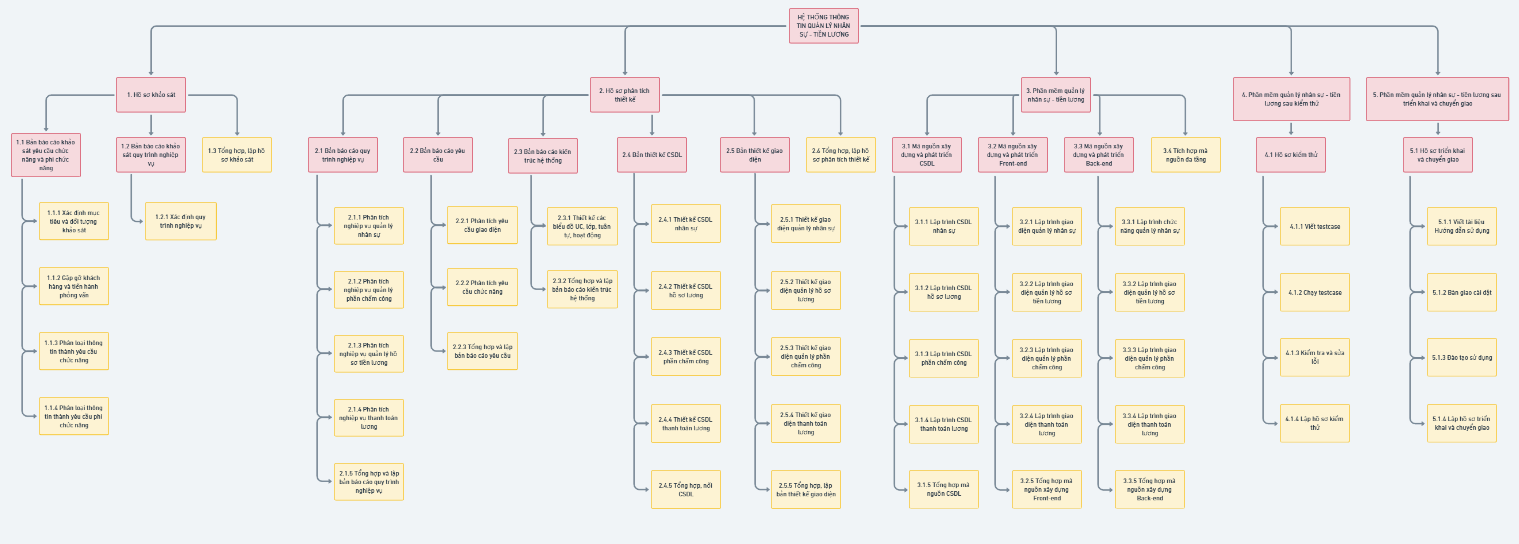
\includegraphics[width=\textwidth]{images/sodophanratongquat.png}
    \caption{Sơ đồ phân rã công việc}
\end{figure}
\begin{figure}[H]
    \centering
    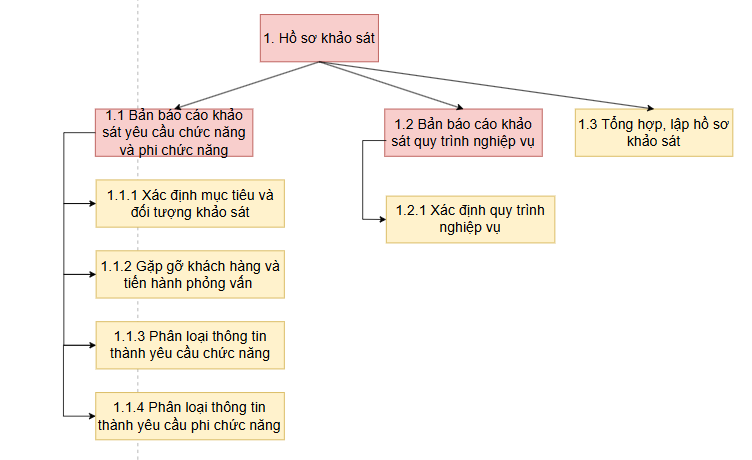
\includegraphics[width=\textwidth]{images/hskhaosat.png}
    \caption{Phân rã chi tiết Hồ sơ khảo sát}
\end{figure}
\begin{figure}[H]
    \centering
    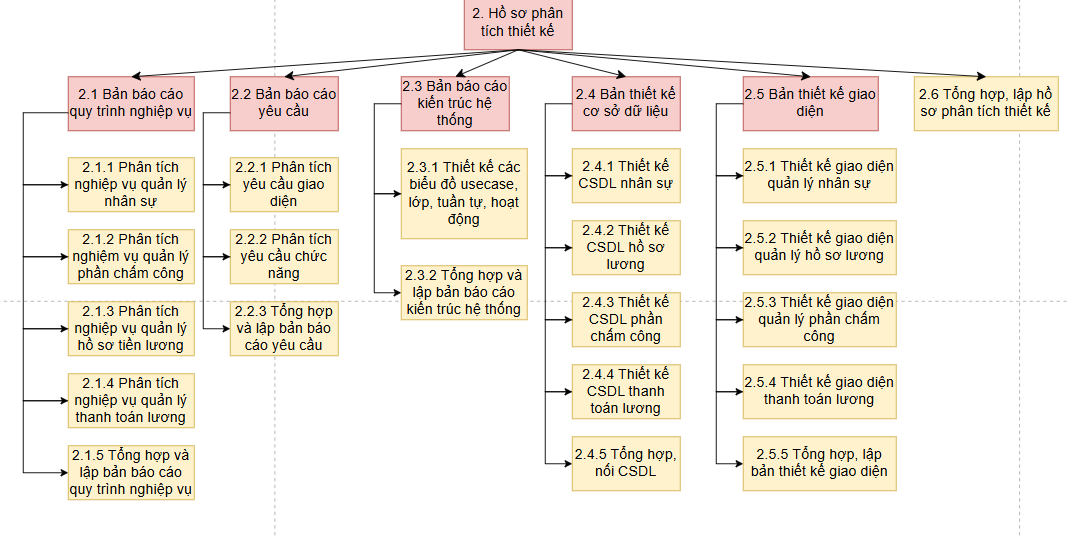
\includegraphics[width=\textwidth]{images/hspttk.png}
    \caption{Phân rã chi tiết hồ sơ phân tích thiết kế}
\end{figure}
\begin{figure}[H]
    \centering
    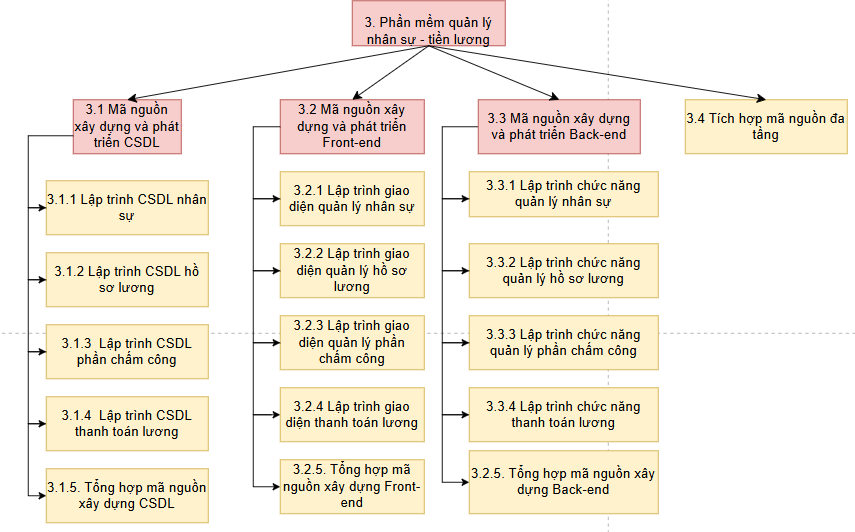
\includegraphics[width=\textwidth]{images/pmquanlyns-tl.png}
    \caption{Phân rã chi tiết phần mềm quản lý nhân sự - tiền lương}
\end{figure}
\begin{figure}[H]
    \centering
    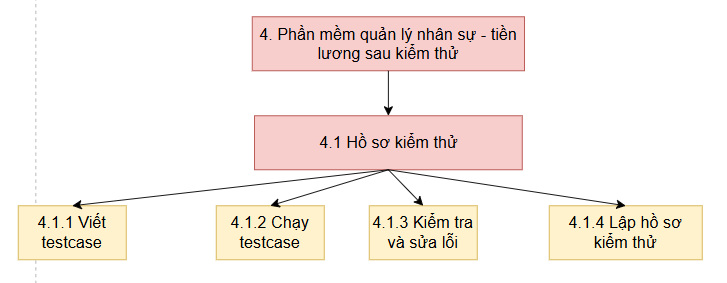
\includegraphics[width=\textwidth]{images/pmsaukiemthu.png}
    \caption{Phân rã chi tiết phần mềm quản lý nhân sự - tiền lương sau kiểm thử}
\end{figure}
\begin{figure}[H]
    \centering
    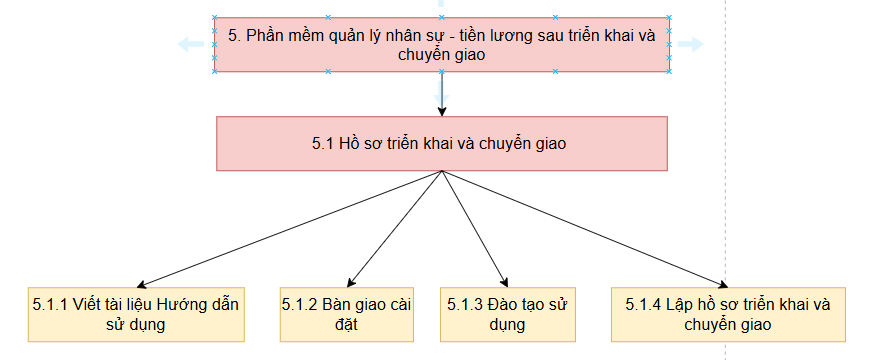
\includegraphics[width=\textwidth]{images/pmsautrienkhai.png}
    \caption{Phân rã chi tiết phần mềm quản lý nhân sự - tiền lương sau triển khai và chuyển giao}
\end{figure}
\subsection{Biên bản phạm vi công việc}
\subsubsection{Xác định mục tiêu và đối tượng khảo sát}
% Viết biên bản phạm vi công việc
\section{Kế hoạch quản lý thời gian}
\subsection{Bảng phụ thuộc công việc và quan hệ thời gian}
% Viết bảng phụ thuộc
\subsection{Sơ đồ AOA và AON}
\subsubsection{Sơ đồ AOA}
\begin{figure}[H]
    \centering
    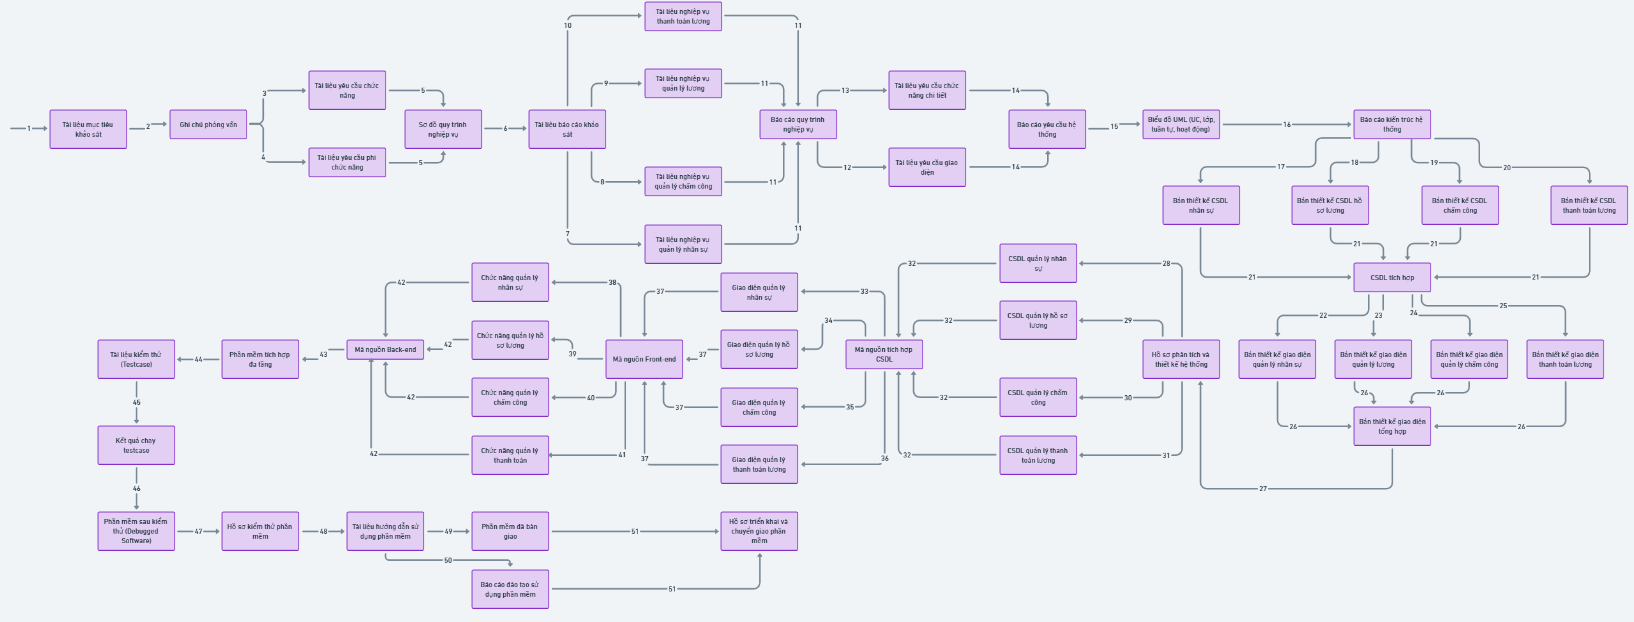
\includegraphics[width=\textwidth]{images/aoa.png}
    \caption{Sơ đồ AOA}
\end{figure}
\subsubsection{Sơ đồ AON}
\begin{figure}[H]
    \centering
    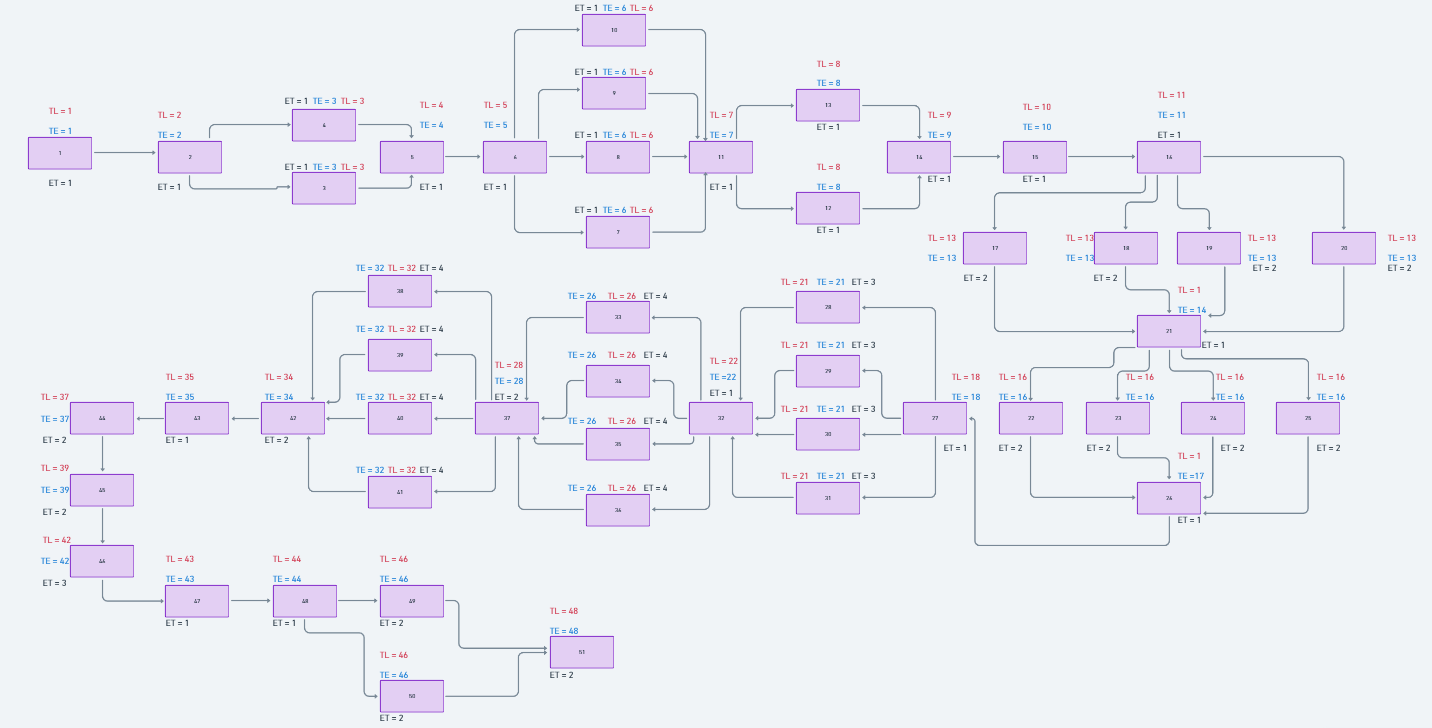
\includegraphics[width=\textwidth]{images/aon.png}
    \caption{Sơ đồ AON}
\end{figure}
\subsection{Sơ đồ Gantt}
\begin{figure}[H]
    \centering
    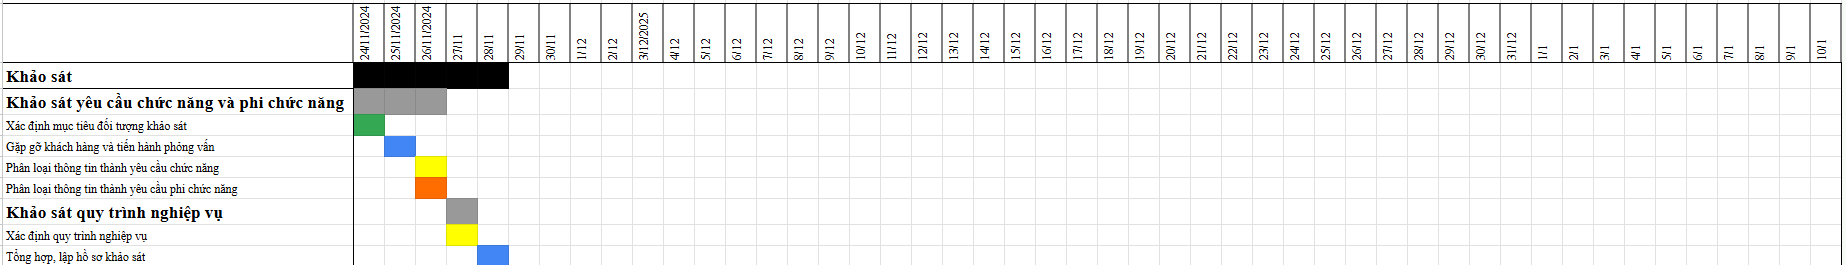
\includegraphics[width=\textwidth]{images/gantt1.png}
    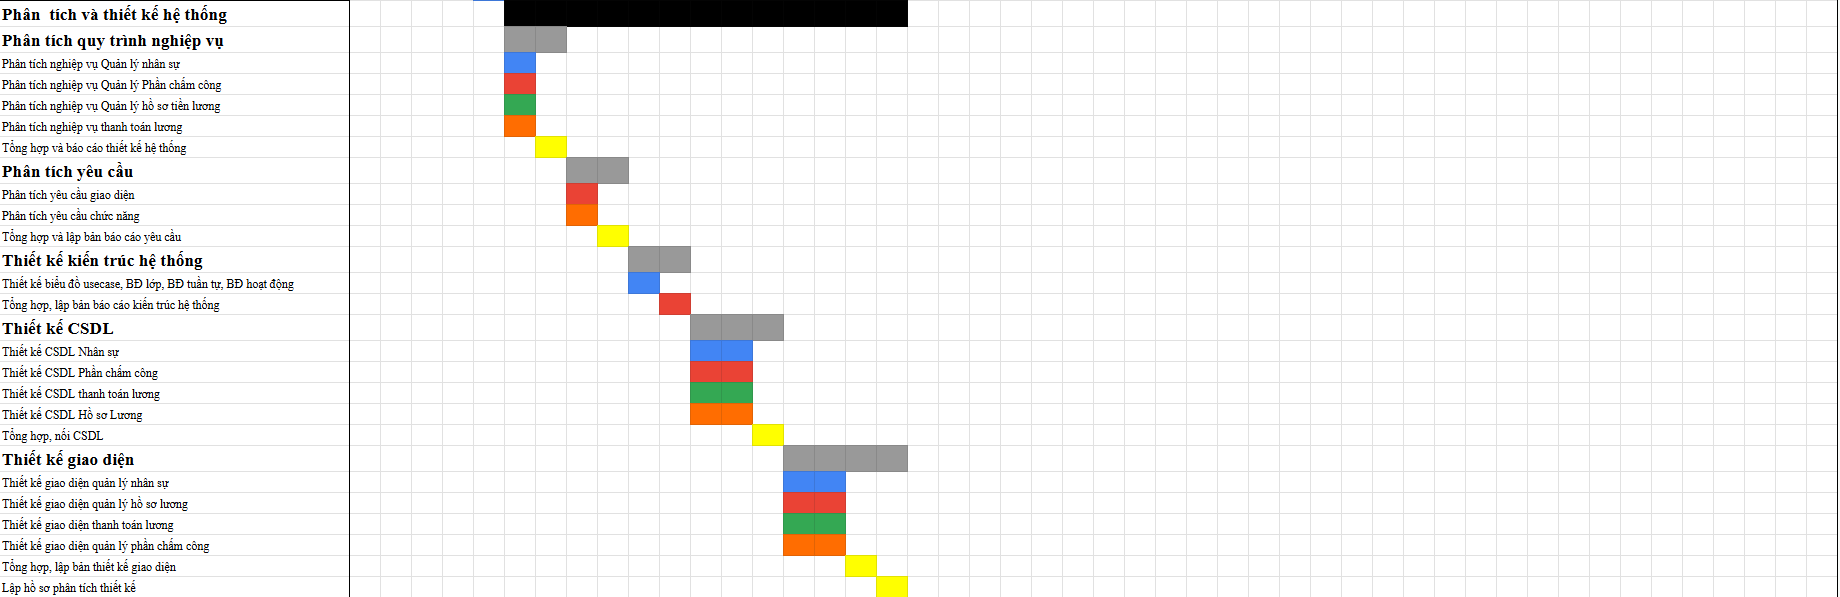
\includegraphics[width=\textwidth]{images/gantt2.png}
    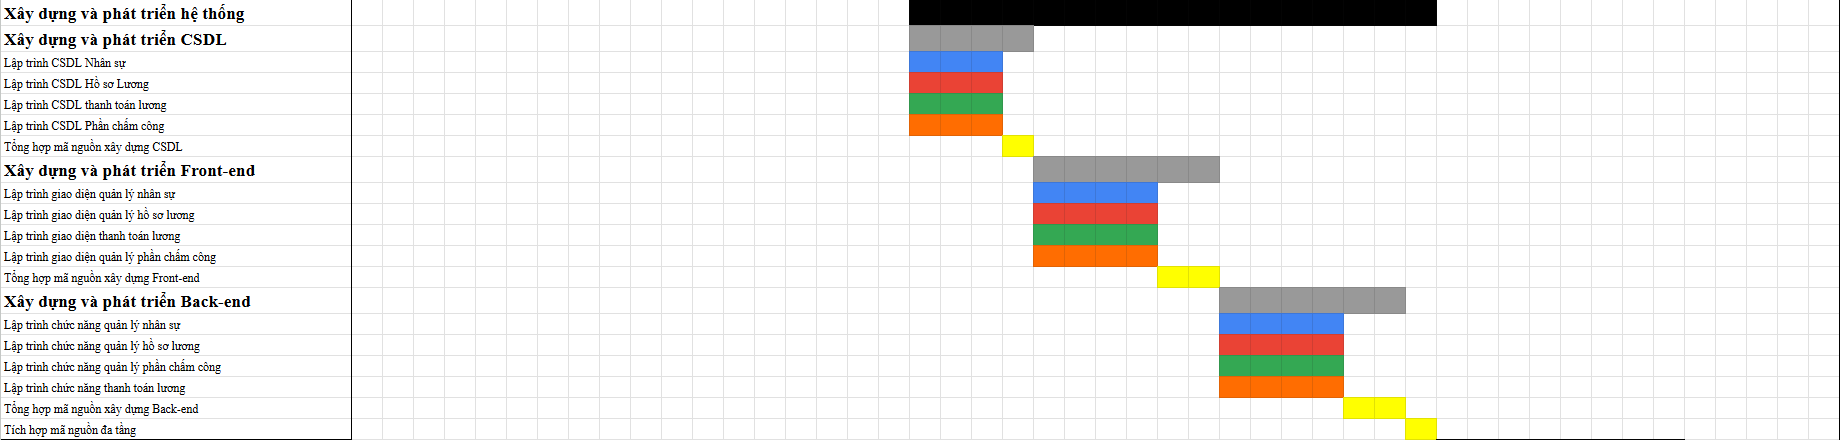
\includegraphics[width=\textwidth]{images/gantt3.png}
    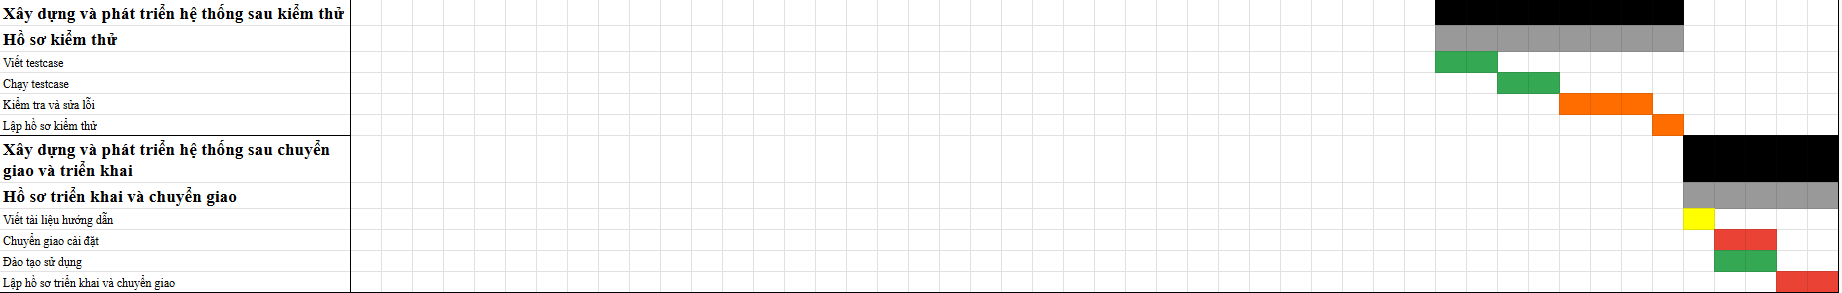
\includegraphics[width=\textwidth]{images/gantt4.png}
    \caption{Sơ đồ Gantt}
\end{figure}
\begin{figure}[H]
    \centering
    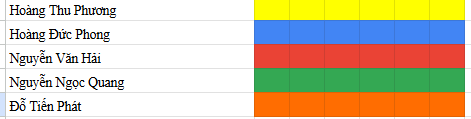
\includegraphics[width=\textwidth]{images/gantt_tv.png}
\end{figure}
\subsection{Tổng kết kế hoạch quản lý thời gian}
% Viết bảng kế hoạch